\chapter{Estado del Arte}

% ********************************************************************

\vspace{-0.3cm}

En este capítulo se llevará a cabo un primer acercamiento a los problemas de seguridad actuales en los sistemas Linux y se introducirán los fundamentos del marco táctico de MITRE \gls{ATT&CK}. También se realizará un análisis de las principales ventajas que está trayendo consigo el uso de la \gls{IA} para la detección de vectores de ataque, y por último se explicará cómo funcionan los \gls{SIEM} más vanguardistas.

\vspace{0.3cm}

\section{Seguridad en sistemas operativos Linux}

Las distribuciones Linux son con un 47\% \cite{linux-stats}, tal y como se indica en la gráfica de la Figura \ref{fig:linux-stats}, una de las principales elecciones para las personas que trabajan en el sector tecnológico. Son muchas las ventajas frente a sus principales competidores, como la posibilidad de adaptación y modificación tan amplia, permitiendo personalizar por completo el entorno de trabajo. Otro factor diferencial es que es de código abierto, y su descarga y uso son totalmente gratuitos, abaratando costes y permitiendo un uso escalable para las empresas e instituciones.

\begin{figure}[H]
    \vspace{-0.2cm}
    \centering
    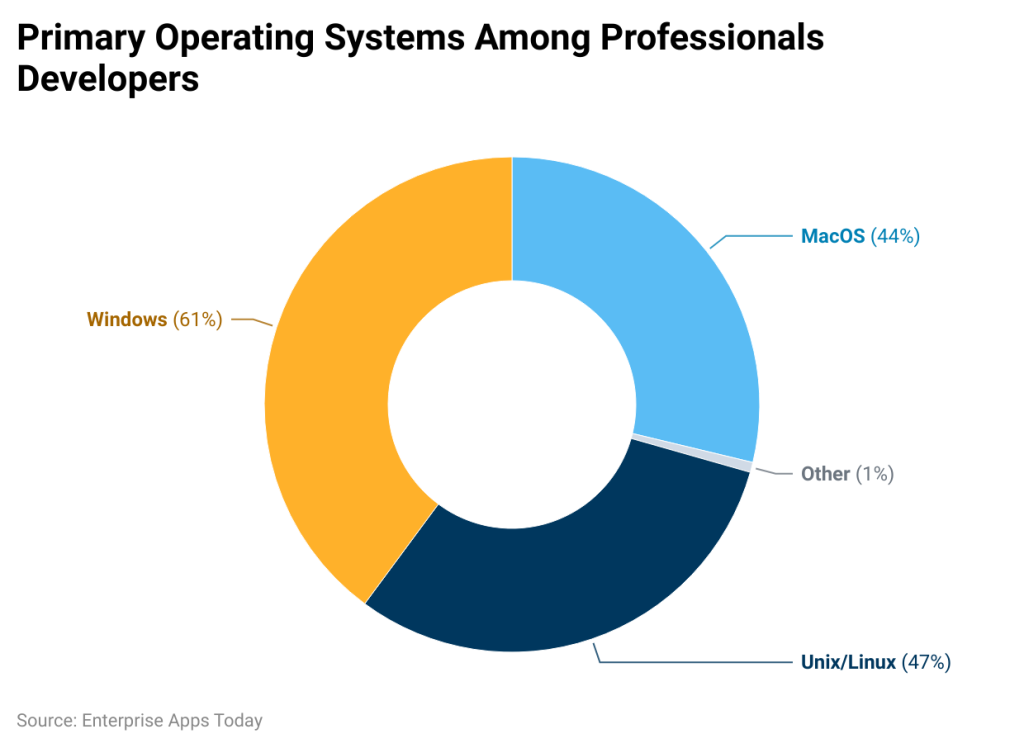
\includegraphics[scale=0.245]{imagenes/primary-operating-systems-among-professionals-developers.png}
    \caption{Comparativa entre sistemas operativos usados por profesionales \cite{linux-stats}}
    \label{fig:linux-stats}
\end{figure}

Dentro del sector de la ciberseguridad, destaca por sus distribuciones orientadas al \textit{pentesting} como \textit{Kali Linux} \cite{kali-linux}, \textit{ParrotOS} \cite{parrotsec-os} o \textit{BlackArch} \cite{blackarch-linux}. 

\vspace{-4mm}

\subsubsection*{Sistema de Archivos de Linux}

El sistema de archivos de Linux (\ref{tab:linux_file_systems}) se distingue por tener una estructura altamente organizada en base a la funcionalidad de los directorios. Entre estos, los ficheros de registro, que son críticos para la seguridad y el diagnóstico del sistema, se almacenan sistemáticamente en \texttt{/var/log}, de modo que las todas las actividades y eventos del sistema sean rastreados detalladamente y mapeados en función de una serie de características.

\begin{table}[H]
\centering
\footnotesize
\begin{tabularx}{\textwidth}{|l|X|}
\hline
\rowcolor{graylight}\texttt{Directorio} & \texttt{Descripción} \\
\hline
/bin & Binarios de comandos esenciales \\
\hline
/boot & Archivos del cargador de arranque del sistema \\
\hline
/dev & Archivos de dispositivo \\
\hline
/etc & Archivos de configuración específicos del host \\
\hline
/home & Directorio de inicio del usuario \\
\hline
/lib & Módulos de biblioteca compartida \\
\hline
/media & Archivos de medios como \textit{CD-ROM} \\
\hline
/mnt & Sistemas de archivos montados temporalmente \\
\hline
/opt & Paquetes de software de aplicaciones adicionales \\
\hline
/proc & Sistema de archivos generado automáticamente \\
\hline
/root & Directorio de inicio del usuario root \\
\hline
/run & Datos del programa en tiempo de ejecución \\
\hline
/sbin & Binarios del sistema \\
\hline
/srv & Datos específicos del sitio servidos por este sistema \\
\hline
/sys & Directorio virtual que proporciona información del sistema \\
\hline
/tmp & Archivos temporales \\
\hline
/usr & Archivos de usuario solo lectura \\
\hline
/var & Archivos que se esperan cambien continuamente \\
\hline
\end{tabularx}
\caption{Estructura del sistema de archivos de SOs basados en Linux}
\label{tab:linux_file_systems}
\end{table}

% ********************************

\subsubsection*{Gestión de permisos en Linux}

Una de las principales ventajas de los sistemas Linux es la gestión de permisos, que se desglosa en tres categorías de usuario. Este modelo divide los derechos de acceso entre el usuario (propietario del archivo), el grupo (otros usuarios que pertenecen al mismo grupo que el archivo) y otros (todos los demás usuarios del sistema). Cada archivo y directorio tiene un conjunto de permisos asociados para estas tres categorías, lo que permite un control granular sobre quién puede leer, escribir o ejecutar un archivo en el sistema.

Los permisos en Linux se identifican comúnmente como lectura (\texttt{r}), escritura (\texttt{w}) y ejecución (\texttt{x}) tal y como se indica en la siguiente tabla (\ref{tab:unix_permissions}). Además, Linux permite el uso de mecanismos avanzados como los permisos \texttt{setuid} y \texttt{setgid}, que otorgan a los programas la capacidad de ejecutarse con los privilegios de otro usuario o grupo, respectivamente. Estos permisos se pueden asignar por medio del comando \texttt{chmod} \cite{chmod-quickref}. Además, los permisos también pueden estar asociados a un fichero específico o a su nivel de pertenencia (\ref{tab:file_types_owners}).

\begin{center}
    \begin{mdframed}
    \scriptsize
            \begin{minted}{bash}
-rwxr-xr-- 22 root 4096 2024-03-03 18:09 file.txt
            \end{minted}
    \end{mdframed}
\end{center}

En este ejemplo, el archivo tiene:
\begin{itemize}
    \item Permisos de lectura, escritura y ejecución para el usuario propietario (rwx)
    \item Permisos de lectura y ejecución para el grupo (r-x)
    \item Solo permisos de lectura para otros usuarios (r--)
\end{itemize}

\begin{table}[H]
\footnotesize
\centering
\renewcommand{\arraystretch}{1.5}
\begin{tabularx}{\textwidth}{|c|c|X|}
\hline
\rowcolor{graylight}\texttt{Abreviatura} & \texttt{Valor} & \textt{Acción} \\
\hline
r & 4 & Lectura \\
w & 2 & Escritura \\
x & 1 & Ejecución \\
- & 0 & Sin permiso \\
\hline
\end{tabularx}
\caption{Estructura de permisos en Sistemas Linux \cite{chmod-quickref}}
\label{tab:unix_permissions}
\end{table}


\begin{table}[H]
\footnotesize
\centering
\renewcommand{\arraystretch}{1.5}
\begin{tabularx}{\textwidth}{|c|X|c|X|}
\hline
\rowcolor{graylight}\texttt{Quién} & \texttt{Significado} & \texttt{Tipo de Archivo Abreviatura} & \texttt{Tipo de Archivo} \\
\hline
u & Usuario & d & Directorio \\
g & Grupo & - & Archivo regular \\
o & Otros & l & Enlace simbólico \\
a & Todos (\texttt{ugo}) & - & -- \\
\hline
\end{tabularx}
\caption{Tipos y propietarios de archivos en Sistemas Linux \cite{chmod-quickref}}
\label{tab:file_types_owners}
\end{table}


Es crucial implementar la política de mínima permisibilidad en la gestión de permisos para minimizar los riesgos de ataques que exploten las estructuras de permisos laxos. Limitar el acceso a la información y funcionalidades del sistema solo a quienes realmente lo necesitan ayuda a proteger contra amenazas internas y externas, y es especialmente importante para evitar que los ataques se propaguen a través de la cadena de mando en un organigrama empresarial.

% ********************************

\subsection{\textit{Hardening} del sistema}

Existen una serie de medidas básicas de seguridad \cite{urrego2023seguridad} para añadir una capa de protección a los Sistemas Linux, y que desgraciadamente no suelen llevarse a cabo por desconocimiento, incluso por aquellos profesionales que despliegan sus servidores y acaban siendo atacados a causa de este motivo. Entre estas medidas, destacan:

\begin{enumerate}[label=\Alph*.,itemsep=2pt,parsep=1pt]
    \item \texttt{Configuración de conexión remota SSH:} cambiar el puerto predeterminado, sustituir el acceso por contraseña por el uso de pares de claves publica-privada y deshabilitar el acceso root directo.
    \vspace{1mm}
    \item \texttt{Listar puertos abiertos:} revisar y filtrar los puertos abiertos para mantener solo los necesarios para la operación segura del sistema. \\
    \item \texttt{Habilitar IPTABLES:} configuración de un \textit{firewall} para controlar el acceso a los servicios según las necesidades de seguridad. \\
    \item \texttt{Prevención de Ataques \gls{DDoS}} (\textit{Distributed Denial-of-Service}): implementación de medidas para mitigar ataques de este tipo, como limitar conexiones y usar SYN cookies. \\
    \item \texttt{Software Instalado:} gestión de los paquetes instalados para asegurar que solo se mantengan los necesarios y se evite software no confiable. \\
    \item \texttt{Actualización Kernel y Parches de Seguridad:} mantener el sistema actualizado con los últimos parches de seguridad para proteger contra vulnerabilidades conocidas. \\
    \item \texttt{Password aging:} implementación de políticas de caducidad y renovación de contraseñas para mejorar la seguridad de las cuentas. \\
    \item \texttt{Encriptación de disco duro:} aplicación de cifrado al nivel de disco para proteger los datos en caso de acceso físico no autorizado. \\
    \item \texttt{Antivirus:} uso de software antivirus para detectar y prevenir malware y otros tipos de software malicioso. \\
    \item \texttt{Uso de \gls{VPN}} (\textit{Virtual Private Network}): conexión a redes privadas virtuales para asegurar las conexiones remotas y proteger los datos en tránsito. \\
    \item \texttt{Servidor de archivos \gls{NFS}:} configuración segura de servidores de archivos en red para compartir recursos dentro de una red de confianza. \\
    \item \texttt{Habilitar \texttt{\gls{SUDO}}:} control de los privilegios de ejecución de comandos para limitar las operaciones que los usuarios pueden realizar. \\
    \item \texttt{Backups:} implementación de copias de seguridad cronológicas para proteger los datos frente a pérdidas accidentales o maliciosas. \\
    \item \texttt{Monitorización y manejo de \textit{logs}:} revisión y análisis de \textit{logs} para detectar actividades inusuales y potenciales brechas de seguridad.
\end{enumerate}

De todas las medidas anteriores, este proyecto estará enfocado en la última: monitorización y manejo de \textit{logs}, con el fin de detectar posible patrones de ataque en base al análisis de los eventos registrados en un sistema o conjunto de sistemas Linux. Igualmente, cada una de ellas representan una capa de robustez en el nivel de seguridad de equipo, por lo que su importancia debe ser tenida en cuenta.

% ********************************

\vspace{-0.3cm}

\subsection{Generación y monitorización de logs}

Los logs son ficheros que registran actividades realizadas en un sistema o servicio. Por consiguiente, estos pueden llegar a ser nuestros principales aliados para detectar intentos de acceso no autorizados, manipulación de datos o incluso intentos de intrusión. Además, proporcionan evidencia crucial en caso de incidentes de seguridad, ayudando en las investigaciones forenses digitales.

Existen diversas herramientas y soluciones para la generación, monitorización y gestión de \textit{logs} que automatizan y facilitan estas tareas. Entre las más destacadas se encuentran: \\

\texttt{\gls{ELK} Stack} (\textit{Elasticsearch, Logstash, y Kibana}) \cite{elastic-stack}: esta suite de herramientas permite la recopilación, indexación, y visualización de \textit{logs} de manera eficiente y escalable. \textit{Elasticsearch} indexa los \textit{logs}, \textit{Logstash} los procesa y \textit{Kibana} proporciona una interfaz gráfica para explorar y visualizar los datos.

\texttt{Splunk} \cite{splunk}: otra solución popular que CISCO \cite{cisco} ofrece con capacidades avanzadas de recogida, indexación y análisis de grandes volúmenes de datos en tiempo real. \textit{Splunk} es particularmente apreciado por su potente interfaz de búsqueda y visualización.

\texttt{Zabbix} \cite{zabbix}: además de monitorizar el rendimiento y la disponibilidad, Zabbix es capaz de recoger y analizar \textit{logs} de diversos sistemas y dispositivos, ofreciendo una solución integral para el seguimiento de infraestructuras \gls{IT}. 

\texttt{Syslog} es, según el \texttt{\gls{RFC} 5424} \cite{rfc5424} , una de las herramientas más antiguas y ampliamente utilizadas para la gestión de \textit{logs} en sistemas GNU/Linux. Permite la centralización de \textit{logs} de múltiples sistemas en un servidor \texttt{syslog}. Utiliza niveles de prioridad asignados a los mensajes:

\begin{table}[H]
\centering
\footnotesize
\begin{tabular}{|c|c|p{8.5cm}|}
\hline
\rowcolor{graylight}\texttt{Valor} & \texttt{Prioridad} & \texttt{Descripción} \\
\hline
0 & Emergency & El sistema no se puede usar \\
\hline
1 & Alert & Se debe actuar inmediatamente \\
\hline
2 & Critical & Condiciones críticas \\
\hline
3 & Error & Condiciones de error \\
\hline
4 & Warning & Condiciones de advertencia \\
\hline
5 & Notice & Condición normal pero significativa \\
\hline
6 & Info & Mensajes informativos \\
\hline
7 & Debug & Mensajes de nivel de depuración \\
\hline
\end{tabular}
\caption{Niveles de prioridad de syslog}
\label{tab:syslog_priority}
\end{table}

Además, hace uso de las llamadas \textit{facilities}, una serie de categorías predefinidas que clasifican los logs en función de la parte del sistema operativo que las ha generado, ayudando a organizar los mensajes para facilitar su filtrado y procesamiento.

\newpage

\begin{table}[H]
\centering
\footnotesize
\begin{tabular}{|c|l|p{8cm}|}
\hline
\rowcolor{graylight}\texttt{Código } & \texttt{Keyword} & \texttt{Descripción} \\
\hline
0 & kern & Mensajes del kernel \\
\hline
1 & user & Mensajes a nivel de usuario \\
\hline
2 & mail & Sistema de correo \\
\hline
3 & daemon & Demonios del sistema \\
\hline
4 & auth & Mensajes de seguridad/autenticación \\
\hline
5 & syslog & Mensajes generados internamente por syslogd \\
\hline
6 & lpr & Subsistema de impresora de línea \\
\hline
7 & news & Subsistema de noticias de red \\
\hline
8 & uucp & Subsistema \gls{UUCP} (\textit{Unix to Unix Copy Protocol}) \\
\hline
9 & cron & Subsistema cron \\
\hline
10 & authpriv & Mensajes de seguridad/autenticación privados \\
\hline
11 & ftp & Demonio \gls{FTP} (\textit{File Transfer Protocol}) \\
\hline
12 & ntp & Subsistema \gls{NTP} (\textit{Network Time Protocol}) \\
\hline
13 & security & Auditoría de logs \\
\hline
14 & console & Alerta de logs \\
\hline
15 & solaris-cron & Demonio de planificación \\
\hline
16–23 & local0 – local7 & Facilities usados localmente \\
\hline
\end{tabular}
\caption{\textit{Facilities} de Syslog}
\label{tab:syslog_facilities}
\end{table}

Las implementaciones de \verb|syslog| varían y están adaptadas para diferentes distribuciones de Linux. Por ejemplo, \verb|rsyslog| es más común en distribuciones basadas en Debian, mientras que \verb|syslog-ng| \footnotemark es ampliamente utilizado en distribuciones basadas en RedHat.

Entre las ventajas de \verb|rsyslog| se encuentra su capacidad para manejar grandes volúmenes de datos. Por otro lado, \verb|syslog-ng| destaca por su capacidad de \textit{parsing} y filtrado de \textit{logs} antes de su almacenamiento, lo que facilita una organización más eficiente y una mejor detección de problemas.

\footnotetext{Donde ng hace referencia a \textit{new-generation}}

Según se observa en la Figura \ref{fig:varlog}, estos ficheros se encuentran comúnmente en la ruta \verb|/var/log|, algunos de ellos en subcarpetas asociadas a servicios o programas específicos que cuentan con su propio sistema de monitorización. En cuanto a la nomenclatura utilizada para los ficheros, hay varios que tienen el mismo nombre seguido de la expresión regular \verb|<name>.log.*| donde * es un número que aumenta secuencialmente. Esto se debe a que cuando se completa el espacio máximo utilizable de un fichero se genera otro nuevo con ese mismo tamaño utilizable. Por ejemplo, en el caso de \verb|boot.log| o de \verb|dpkg.log|.

\begin{figure}[H]
    \centering
    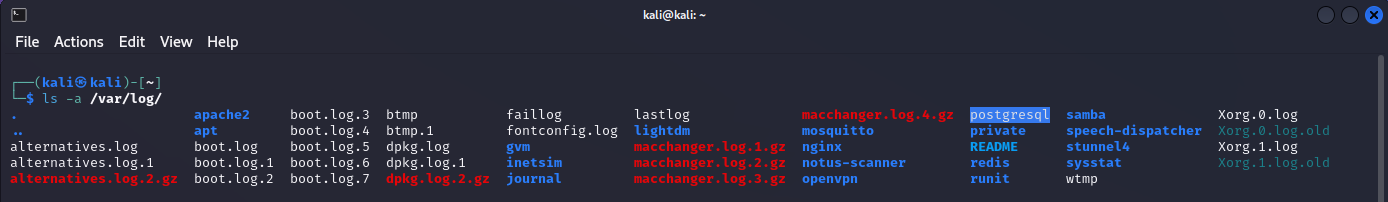
\includegraphics[width=\textwidth]{imagenes/var-log.png}
    \caption{Contenido del registro de \textit{/var/log}}
    \label{fig:varlog}
\end{figure}

\newpage

Los logs pueden presentar diferencias en base a la información que almacenan, al formato y al orden en el que la representan, de modo que inicialmente no resulta sencillo trabajar con dos tipos de ficheros \textit{log} de diferentes formatos. En las siguientes Figuras, se muestra el contenido de \verb|auth.log| y de \verb|dpkg.log| (\ref{fig:auth-log} y \ref{fig:dpkg-log} respectivamente):

\begin{figure}[H]
\centering
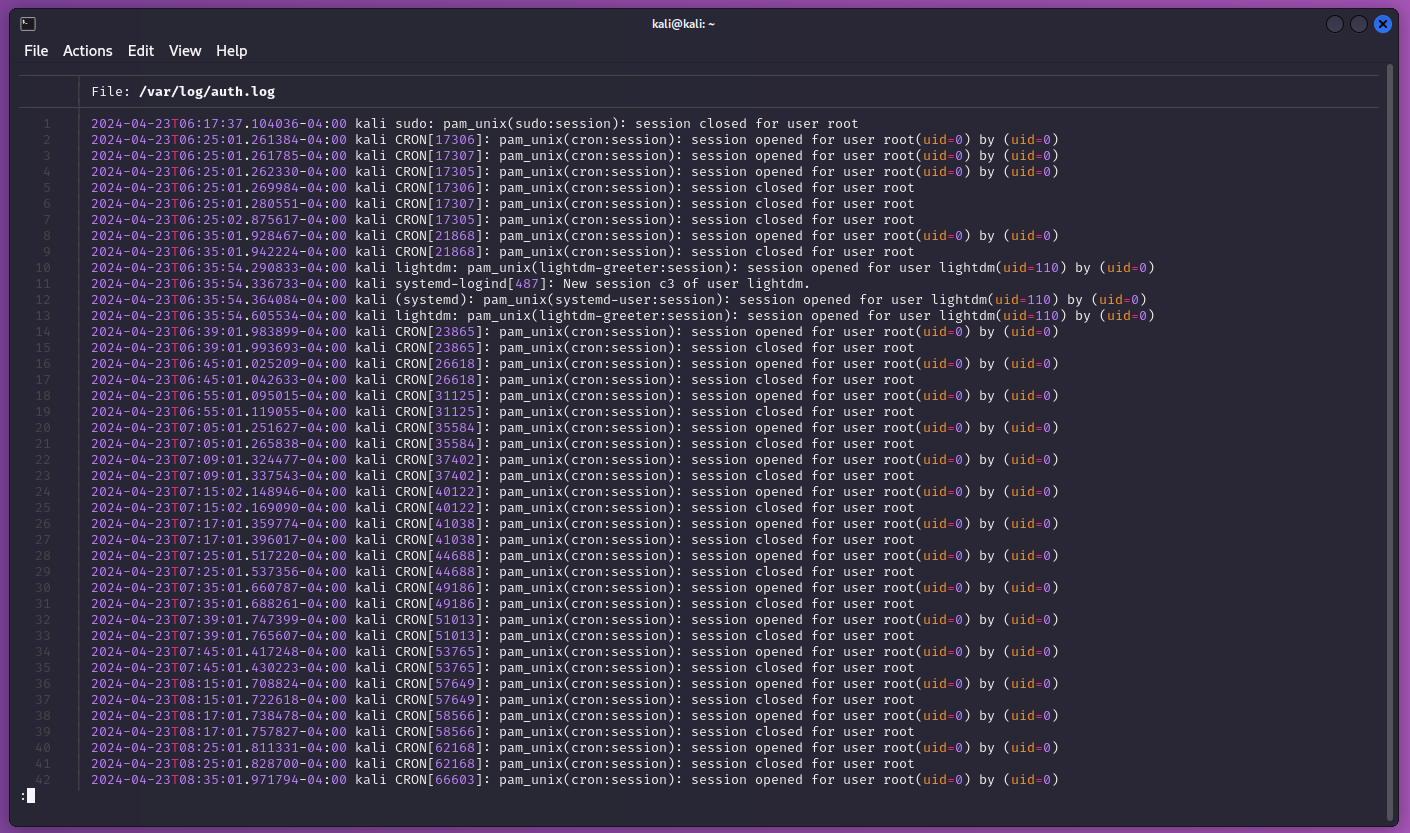
\includegraphics[width=\linewidth]{imagenes/log-structure.png}
\captionof{figure}{Contenido del registro de \textit{auth.log}}
\label{fig:auth-log}
\end{figure}

\begin{figure}[H]
    \centering
    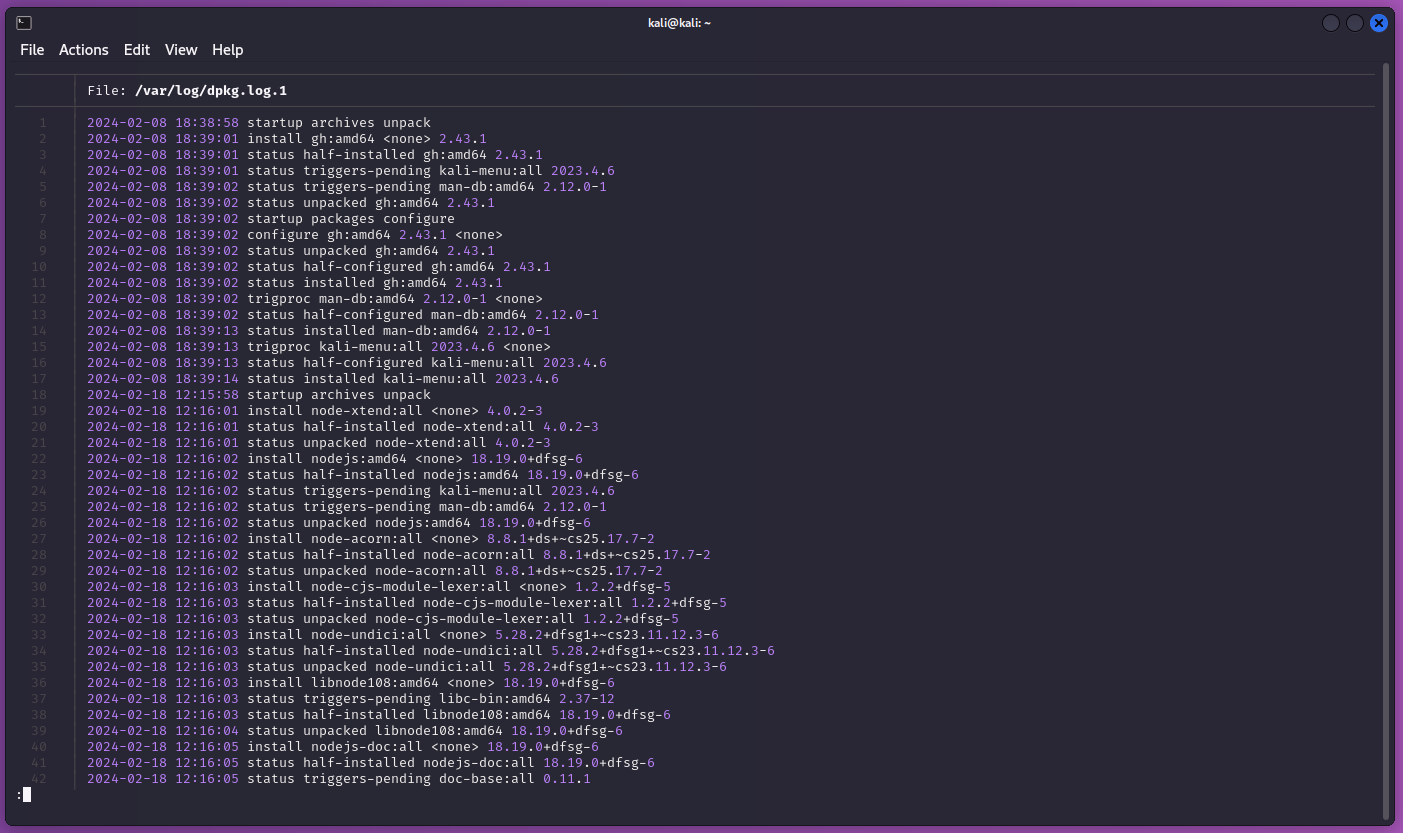
\includegraphics[width=\linewidth]{imagenes/log-structure-2.png}
    \caption{Contenido del registro de \textit{dpkg.log}}
    \label{fig:dpkg-log}
\end{figure}

\newpage

En estos ejemplos, ambos ficheros contienen los campos \textit{timestamp}, es decir, la fecha y la hora a la que sucedió cada evento, y \textit{message}, pero propiedades como la separación entre campos o la precisión que presentan son distintas. A pesar de estas diferencias, la información puede llegar a combinarse a través de técnicas de preprocesamiento de modo que sea utilizable dentro de un mismo formato de \textit{datasets}. 

Además de los ficheros comentados anteriormente, existen otras herramientas importantes para el manejo de \textit{logs} en Linux que contribuyen al análisis de seguridad y al diagnóstico de problemas:

\begin{itemize}
    \item \verb|dmesg|: muestra mensajes del kernel útiles para diagnosticar problemas de hardware y de carga de controladores durante el arranque (puede visualizarse en la Figura \ref{fig:dmesg}).
    \item \verb|journalctl|: herramienta para consultar y administrar \textit{logs} del sistema gestionados por \verb|systemd| (puede visualizarse en la Figura \ref{fig:journalctl}).
\end{itemize}

\begin{figure} [H]
    \centering
    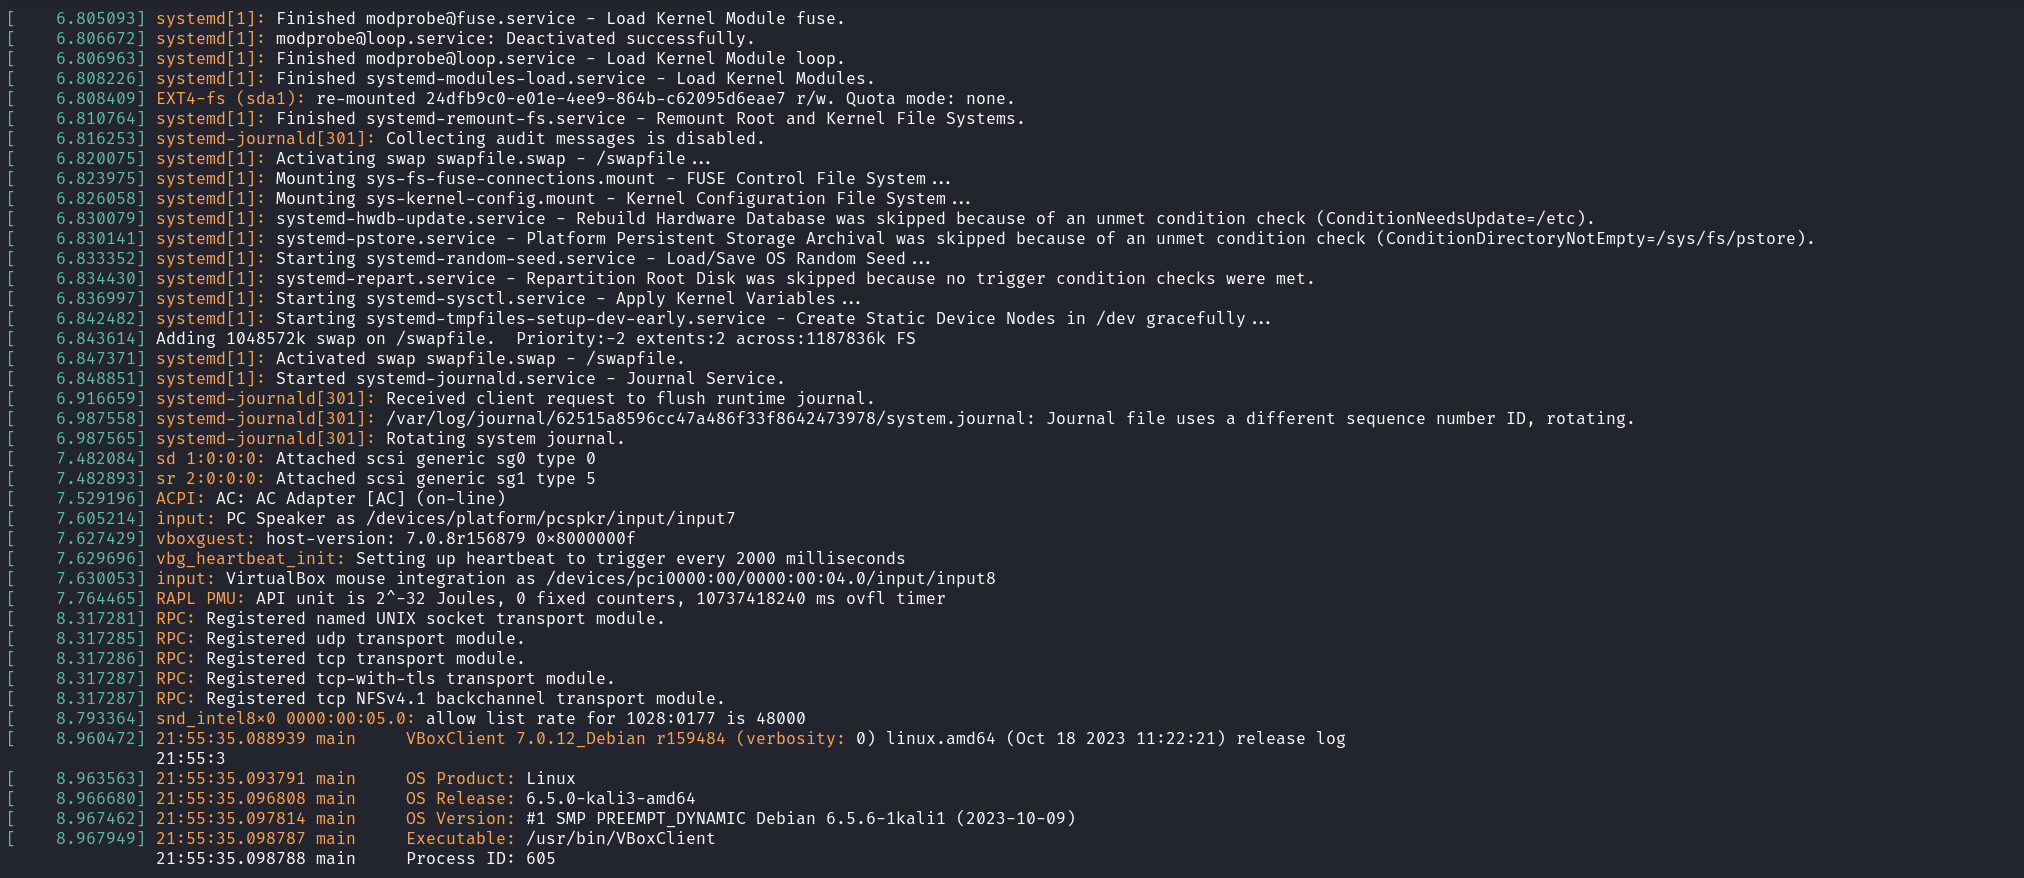
\includegraphics[width=1\linewidth]{imagenes/dmesg.png}
    \caption{Contenido de los logs de \textit{dmesg}}
    \label{fig:dmesg}
\end{figure}

\begin{figure}[H]
    \centering
    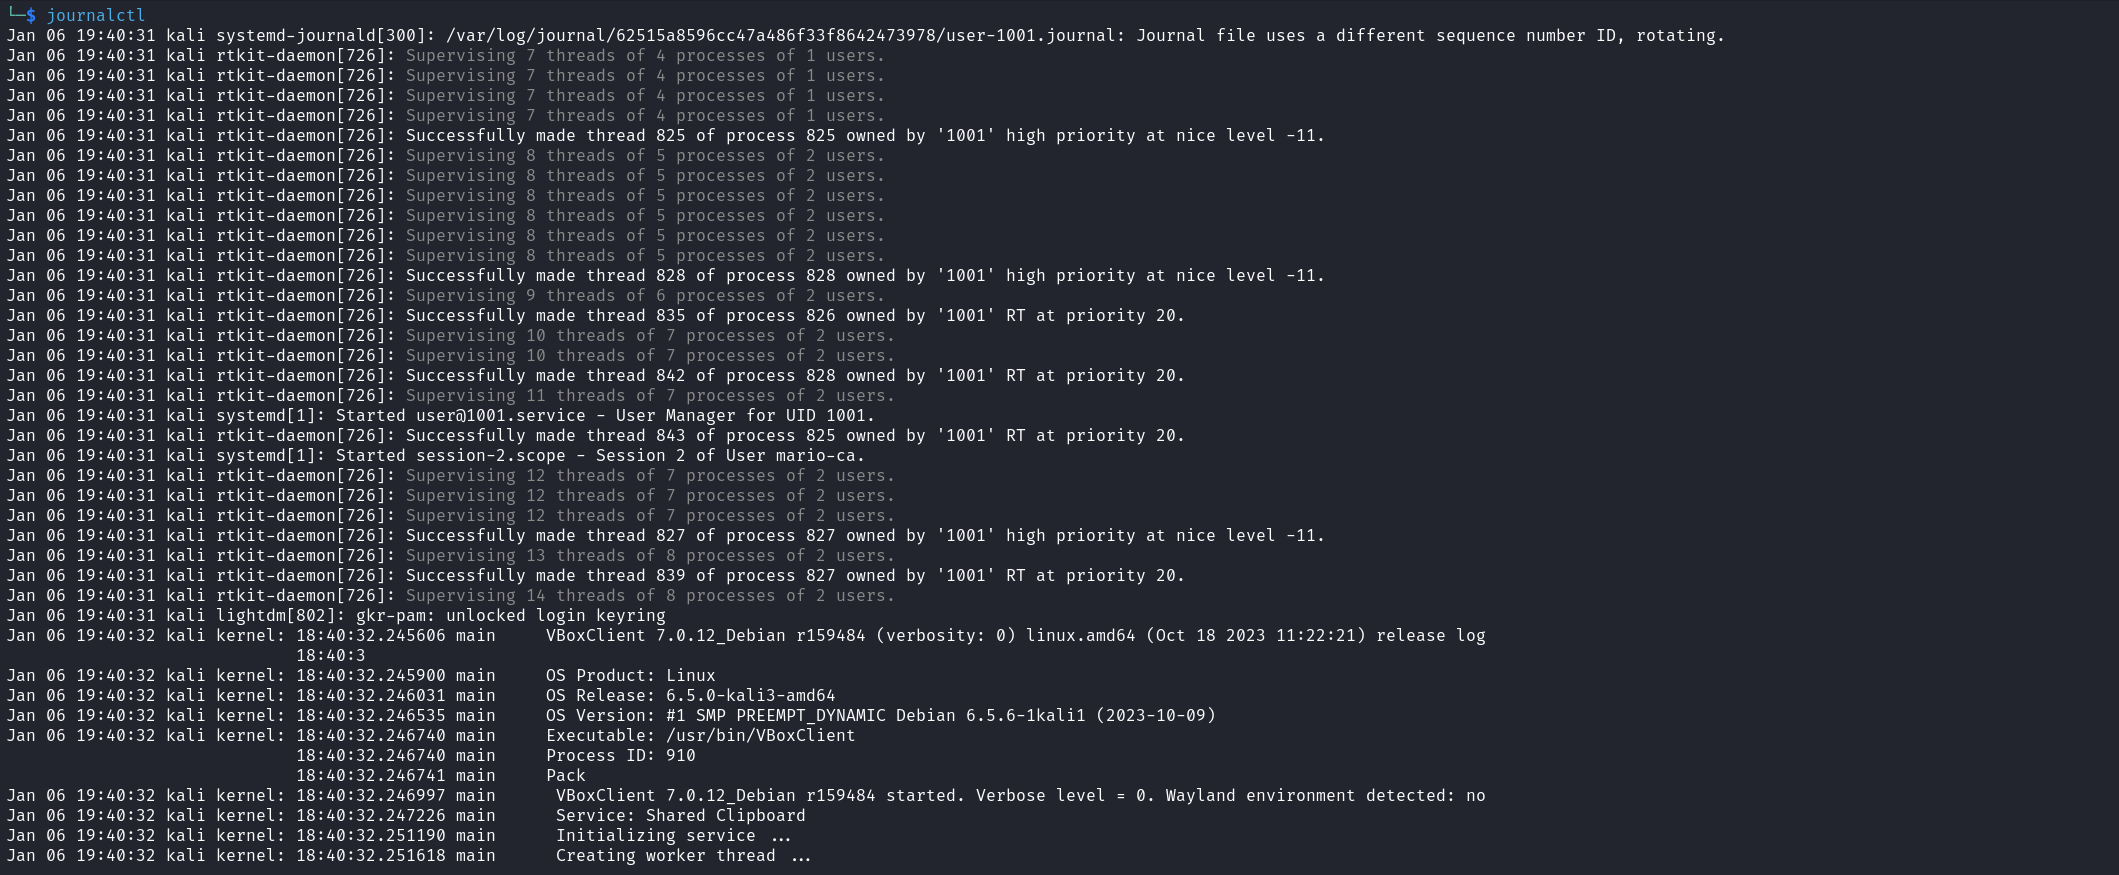
\includegraphics[width=1\linewidth]{imagenes/journalctl.png}
    \caption{Contenido de los logs de \textit{journalctl}}
    \label{fig:journalctl}
\end{figure}

% ********************************

\newpage

% ********************************************************************

\section{El marco de MITRE ATT\&CK}

Con el fin de proporcionar una guía detallada y práctica que permita entender y combatir mejor los ciberataques, nació en 2013 \cite{10005490} el marco de técnicas adversarias de MITRE \gls{ATT&CK} (\textit{Adversarial Tactics, Techniques, and Common Knowledge}). Este fue creado por el \gls{NIST}, y clasifica las diferentes \gls{TTP}s (\textit{Tactics, Techniques and Procedures}) seguidas por los cibercriminales en cada una de las fases de un ataque.

\vspace{-1mm}

\begin{itemize}
    \item \textbf{Tácticas}: Describen el \textit{qué} y el \textit{porqué} de las acciones de los adversarios, refiriéndose a su objetivo general y estrategia durante un ataque.
    \item \textbf{Técnicas}: Revelan el \textit{cómo}, especificando el método específico empleado para alcanzar un objetivo táctico.
    \item \textbf{Procedimientos}: Son los \textit{detalles exactos} de la técnica utilizada, incluyendo los comandos ejecutados, la secuencia de operaciones y cualquier configuración aplicada.
\end{itemize}

\vspace{-1mm}

Por ejemplo, en un ataque de \textit{phishing}, la \textbf{táctica} empleada sería la recopilación inicial de acceso, la técnica podría ser el envío de correos electrónicos engañosos y por último el \textbf{procedimiento} consistiría en el uso de un correo electrónico que aparenta ser una alerta legítima de seguridad de una institución conocida para engañar a los usuarios y hacer que revelen sus credenciales.

MITRE \gls{ATT&CK} está compuesto por una lista estructurada de comportamientos expresados en forma matricial que, tal y como se ilustra en la Figura \ref{fig:mitre-matrix}, proporcionan una taxonomía común de acciones tanto del propio adversario como de contra-medidas para defenderse del mismo.

\vspace{-1mm}

\begin{figure}[H]
    \centering
    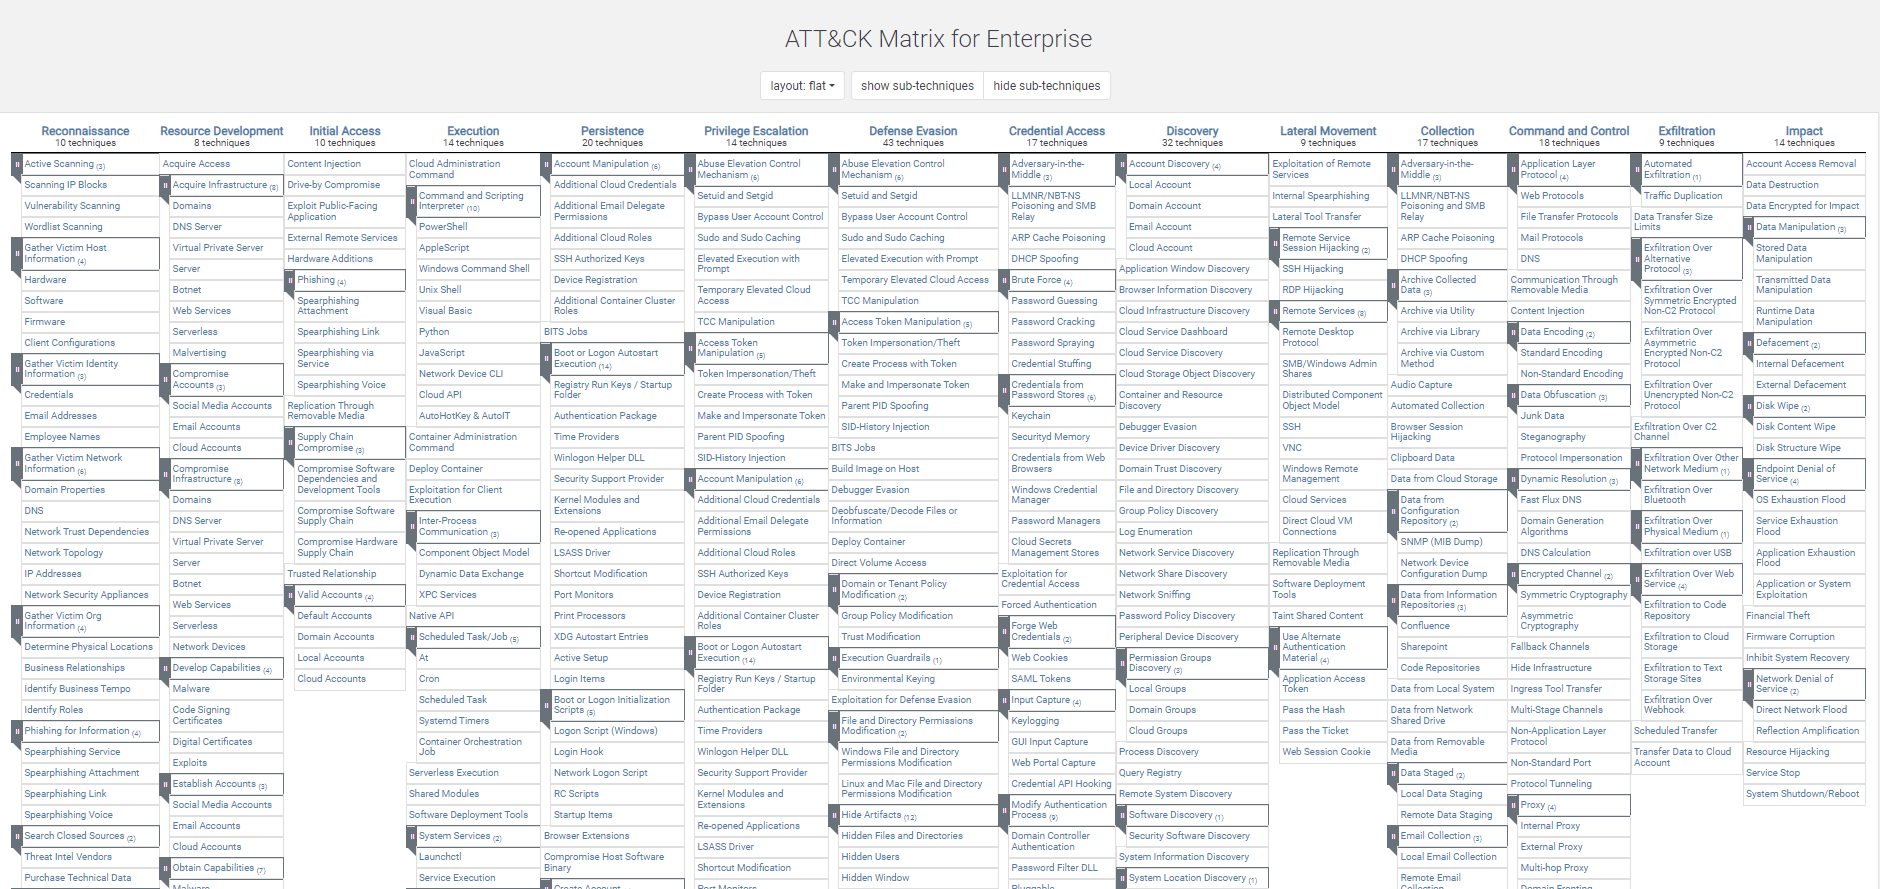
\includegraphics[width=\textwidth]{imagenes/mitre-matrix.png}
    \caption{Matriz de técnicas y tácticas de MITRE ATT\&CK para enterprise \cite{mitre_attack}}
    \label{fig:mitre-matrix}
\end{figure}

\vspace{-2.5mm}

Actualmente es muy utilizado tanto a nivel empresarial como gubernamental a modo de modelo base para el desarrollo de productos y servicios de ciberseguridad. La principal causa de su éxito podría ser la forma en la que se describe cada procedimiento de forma detallada y con una terminología correcta y entendible, pero sin llegar a mencionar el uso de herramientas especificas que lleven a cabo las acciones descritas. 

\newpage

Una gran ventaja de MITRE ATT\&CK \cite{mitre_attack} es que se encuentra en una constante evolución, incorporando a la matriz técnicas y sub-técnicas vanguardistas que van apareciendo en la escena del cibercrimen. Cada una de las técnicas y sub-técnicas \ref{sec:técnicas} de la matriz de MITRE está asociada a un identificador único y cuenta con su correspondiente descripción, además de otra información de relevancia como un listado de formas de mitigación y/o detección. 

Estos identificadores se estructuran siguiendo un patrón muy similar: uno o dos caracteres seguidos de cuatro dígitos. Esta forma de identificarlos permite reservar el suficiente espacio como para añadir durante muchos años nuevas tácticas, técnicas, sub-técnicas, procedimientos, etc.

\begin{table}[h]
\centering
\footnotesize
\begin{tabular}{|c|l|p{8cm}|}
\hline
\rowcolor{graylight}\texttt{Identificador} & \texttt{Categoría} & \texttt{Descripción} \\
\hline
\texttt{TA\#\#\#\#} & Tácticas & TA indica que es un identificador de táctica y va seguido de 4 dígitos. Ejemplo: \texttt{TA0001}. \\
\hline
\texttt{T\#\#\#\#} & Técnicas & T indica que es un identificador de técnica y va seguido de 4 dígitos. Ejemplo: \texttt{T1059}. \\
\hline
\texttt{T\#\#\#\#.\#\#\#} & Sub-técnicas & Parecido a los identificadores de técnicas, pero cuentan con caracteres adicionales ya que se agrupan dentro de los anteriores. Ejemplo: \texttt{T1059.001}. \\
\hline
\texttt{M\#\#\#\#} & Mitigaciones & M indica que es un identificador de mitigación y va seguido de 4 dígitos. Ejemplo: \texttt{M1050}. \\
\hline
\texttt{DS\#\#\#\#} & Detecciones & DS indica que es un identificador de detección y va seguido de 4 dígitos. Ejemplo: \texttt{DS0029}. \\
\hline
\texttt{S\#\#\#\#} | \texttt{G\#\#\#\#} & Procedimientos & Identificadores de procedimientos específicos usados por actores de amenazas o grupos específicos. Ejemplo: \texttt{S0003} para procedimientos y \texttt{G0007} para grupos. \\
\hline
\end{tabular}
\caption{Identificadores del marco de \textit{MITRE ATT\&CK}}
\label{tab:mitre_attack_identifiers}
\end{table}

Hace relativamente poco, se publicaron versiones más específicas de esta matriz tanto para móviles como para \gls{ICS} (\textit{Industrial control system}). Estas contienen menos volumen de tácticas y técnicas pero se adaptan mejor a un escenario real de ataque sobre este tipo de entornos. Además, desde MITRE han desarrollado también matrices específicas para distintos Sistemas Operativos y áreas de conocimiento, también más pequeñas pero más precisas al entorno de simulación.

\begin{table}[h!]
    \footnotesize
    \centering
    \begin{tabularx}{\linewidth}{|l|X|} % Cambio de tipo de columna para mejor control sobre el ancho de la primera columna
        \hline 
        \footnotesize \rowcolor{graylight}\texttt{Categoría} & \footnotesize \texttt{Plataformas / Sistemas} \\ 
        \hline
        \footnotesize \texttt{Enterprise} & 
        \begin{tabular}[t]{@{}l@{}}
            PRE \\
            Windows \\
            macOS \\
            Linux \\
            Cloud \\
            Network \\
            Containers \\
        \end{tabular} \\
        \hline
        \footnotesize \texttt{Mobile} &
        \begin{tabular}[t]{@{}l@{}}
            Android \\
            iOS \\
        \end{tabular} \\
        \hline
        \footnotesize \texttt{ICS} & 
        \begin{tabular}[t]{@{}l@{}}
            \gls{PLC}, \gls{RTU}, \gls{SCADA}, \gls{DCS} 
        \end{tabular} \\
        \hline
    \end{tabularx}
    \caption{Matrices de MITRE ATT\&CK}
    \label{tab:mitre_attack_matrices}
\end{table}


En el caso de este proyecto se hará uso de la matriz de Linux ya que es la que mejor se adapta al escenario donde se llevarán a cabo las simulaciones de ataques.

\subsection{Tácticas} \label{sec:tacticas}

MITRE ATT\&CK  \cite{mitre_attack} agrupa las distintas técnicas de intrusión dentro de catorce tácticas distintas ordenadas secuencialmente, aunque este orden puede orden variar en determinadas operaciones.

\begin{table}[H] 
\centering
\footnotesize
\begin{tabular}{|c|l|p{8cm}|}
\hline
\rowcolor{graylight}\texttt{Código} & \texttt{Fase del Ataque} & \texttt{Descripción} \\
\hline
1 & Reconocimiento & Recopilación de información para la planificación futura un ataque. \\
\hline
2 & Desarrollo de recursos & Creación de recursos que respalden el desarrollo de un ataque. \\
\hline
3 & Acceso inicial & Intento inicial de acceder al objetivo a comprometer. \\
\hline
4 & Ejecución & Introducción de código malicioso en el sistema atacado. \\
\hline
5 & Persistencia & Asentar un acceso continuo al sistema objetivo a través de reinicios, cambios de credenciales y supresión de interrupciones que podrían cancelar su acceso. \\
\hline
6 & Escalada de privilegios & Obtención de permisos de nivel superior para poder acceder a más recursos del sistema atacado. \\
\hline
7 & Evasión de defensa & Ocultación frente a la detección mientras se está efectuando la operación de compromiso. \\
\hline
8 & Acceso a credenciales & Robo de credenciales para acceder al sistema de destino. \\
\hline
9 & Descubrimiento & Obtención de más conocimientos sobre el sistema objetivo y su entorno. \\
\hline
10 & Movimiento lateral & Desplazamiento a través del entorno interno del conjunto de sistemas objetivo. \\
\hline
11 & Recopilación & Búsqueda de información relevante del objetivo. \\
\hline
12 & \gls{C2} - Command \& Control & Comunicación remota con el sistema comprometido para controlar y operar sobre este. \\
\hline
13 & Exfiltración & Robo de datos sensibles almacenados en el sistema comprometido. \\
\hline
14 & Impacto & Manipulación, ocultación o destrucción del sistema comprometido y sus datos. \\
\hline
\end{tabular}
\caption{Conjunto de tácticas ofensivas del marco de \textit{MITRE ATT\&CK}}
\label{tab:mitre_attack_phases}
\end{table}

\subsection{Técnicas} \label{sec:técnicas}

Cada una de las tácticas indicadas en la subsección anterior (\ref{sec:tacticas}) contiene un listado técnicas que pueden utilizarse para llevar a cabo cada objetivo. Estas técnicas a su vez agrupan una serie de subtécnicas, proporcionando un mayor nivel de abstracción que aglutine una mayor base de conocimiento con respecto a todas las formas de llevar a cabo una acción. 

Todo esto puede resultar inicialmente algo confuso de entender, por lo que una manera útil de comprenderlo es imaginarlo como una especie de matriz tridimensional en la que cada táctica es una fila (abscisas), cada técnica una columna (ordenadas) y por último cada subtécnica una altura o cota. Por ejemplo, dentro de la táctica de Reconocimiento (\ref{tab:mitre_attack_phases}) existen actualmente diez técnicas distintas, cada una de ellas con una serie de subtécnicas más específicas.

\begin{figure}[H]
    \centering
    \begin{minipage}[b]{0.45\textwidth}
        \centering
        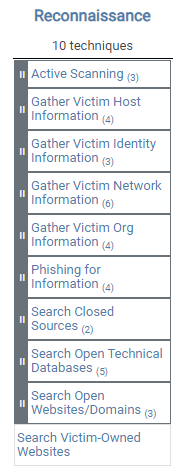
\includegraphics[width=25mm]{imagenes/techniques.png}
        \caption{Listado de técnicas de la táctica de \textit{Reconnaissance} \cite{mitre_attack}}
        \label{fig:reconnaissance-techniques}
    \end{minipage}
    \hspace{0.05\textwidth} % Espacio horizontal entre las dos minipages
    \begin{minipage}[b]{0.45\textwidth}
        \centering
        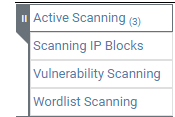
\includegraphics[width=5cm]{imagenes/active-scanning.png}
        \caption{Sub-técnicas de \textit{Active Scanning} \cite{mitre_attack}}
        \label{fig:active-scanning}
    \end{minipage}
\end{figure}


Según se ilustra en las Figuras \ref{fig:reconnaissance-techniques} y \ref{fig:active-scanning}, la primera técnica de la táctica de Reconocimiento, \textit{Active Scanning}, cuenta con 3 subtécnicas: \textit{Scanning IP Blocks}, \textit{Vulnerability Scanning} y \textit{Wordlist Scanning}.


\subsection{Procedimientos}

Por último, se encuentran los procedimientos, que ofrecen una guía detallada de cómo se han de realizar las las técnicas o subtécnicas. En el ejemplo ilustrado en la Figura \ref{fig:ejemplo-procedimiento}, se explica el procedimiento para realizar escaneos de bloques \gls{IP} como técnica de reconocimiento, en la que los adversarios pueden escanear bloques de direcciones \gls{IP} para recabar información sobre redes objetivo que posteriormente puede ser usada en ataques. Dichos escaneos varían desde \textit{pings} simples hasta métodos más sofisticados que revelan versiones de software hasta otros más sencillos.


\begin{figure}[H]
    \centering
    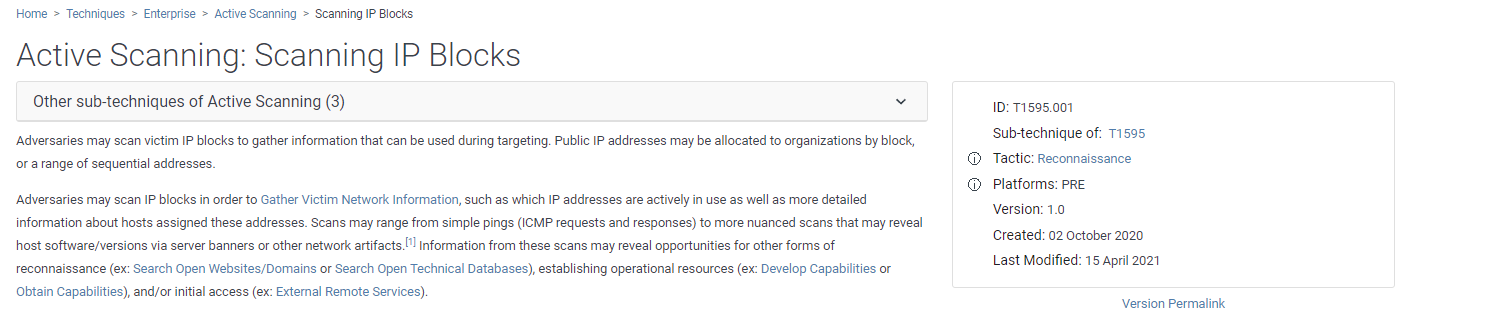
\includegraphics[width=1\linewidth]{imagenes/17.png}
    \caption{Información referente al procedimiento asignado \textit{Scanning \gls{IP}  Blocks} \cite{mitre_attack}}
    \label{fig:ejemplo-procedimiento}
\end{figure}

Adicionalmente, como se observa en la Figura \ref{fig:ejemplo-procedimiento-2}, se puede encontrar justo debajo ejemplos de técnicas de Detección y Mitigación, también identificadas bajo el criterio mencionado anteriormente.

\begin{figure}[H]
    \centering
    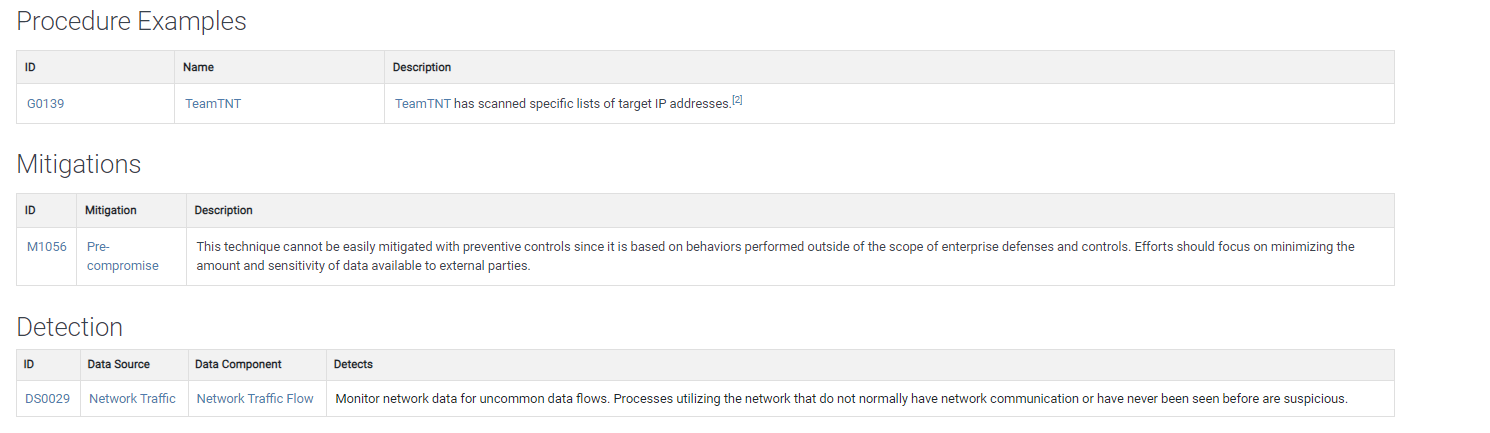
\includegraphics[width=1\linewidth]{imagenes/18.png}
    \caption{Ejemplos de mitigación y detección frente a \textit{Scanning \gls{IP} Blocks} \cite{mitre_attack}}
    \label{fig:ejemplo-procedimiento-2}
\end{figure}

\subsubsection{Frameworks basados en MITRE \gls{ATT&CK}}

Actualmente existen numerosos \textit{frameworks} basados en el marco adversario de MITRE para orquestar simulaciones de ataques en auditorías de seguridad tanto internas como externas. Algunos de estos \textit{frameworks} son:

\begin{itemize}
    \label{frameworks-mitre}
    \item \texttt{\gls{CALDERA}} \cite{caldera}: Desarrollado por el propio MITRE, este \textit{framework} permite planificar, ejecutar y evaluar campañas adversarias basadas en las técnicas definidas en la matriz de \gls{ATT&CK}. Con más de 800 artículos y libros publicados en plataformas académicas como Google Scholar y Scopus, puede considerarse el más utilizado en la actualidad y por tanto el elegido para la implementación de este proyecto, por lo que será explicado con mayor detalle en secciones posteriores.
    \vspace{0.5mm}
    \item \texttt{Red Team Automation (\gls{RTA})} \cite{rta}: Un conjunto de \textit{scripts} diseñados para generar tráfico malicioso que simula comportamientos específicos basados en MITRE \gls{ATT&CK}.  
    \vspace{0.5mm}
    \item \texttt{Atomic Red Team} \cite{atomic_red_team}: Es un conjunto de pruebas pequeñas y altamente portátiles, cada una diseñada para ejecutar una técnica única de MITRE \gls{ATT&CK}. Es útil para equipos de seguridad que desean probar sus defensas de manera incremental y sistemática.
    \vspace{0.5mm}
    \item \texttt{Infection Monkey} \cite{infection_monkey}: Una herramienta de seguridad de código abierto que simula ataques en la red para probar la resiliencia de los sistemas y la eficacia de las medidas de defensa en profundidad. Utiliza técnicas de MITRE \gls{ATT&CK} para evaluar cómo los adversarios podrían avanzar dentro de la red.
    \vspace{0.5mm}
    \item \texttt{Scythe} \cite{scythe}: Esta plataforma permite a los usuarios crear y ejecutar campañas de simulación de amenazas que replican el comportamiento de los adversarios basado en \gls{ATT&CK}.
\end{itemize}

\newpage

% ********************************************************************

\section{Modelos de IA para la detección de vectores de ataque}

Es innegable que en todos los campos tecnológicos se quiere aprovechar al máximo las novedades que está trayendo consigo la Inteligencia Artificial. Concretamente, en el sector de la ciberseguridad muchas empresas de desarrollo de software están tratando de acoplar el análisis e interpretación de datos masificados a través de modelos de \gls{ML} (\textit{Machine Learning}) y \gls{DL} (\textit{Deep Learning}) con el fin de agilizar diversas tareas que hasta la fecha han tenido que llevarse a cabo manualmente por personas, ocupando gran parte del horario laboral, y por tanto no pudiendo ser invertido en otras actividades en las que el desempeño humano es totalmente necesario para la toma de decisiones.

Es por ello que está incrementando considerablemente la cantidad de artículos científicos y de investigación publicados en los que se exploran distintas técnicas y se realizan pruebas haciendo uso de \textit{datasets} generados de forma natural o sintética.

Además de las propias empresas, es bien conocido que algunos grupos de cibercriminales o grupos de ciberterrorismo que operan a la escala de grandes empresas tienen sus propias áreas de \gls{I+D} (\textit{Investigation \& Development}) en las que investigan cómo a través de la IA \cite{barry2024} pueden refinar ataques a gran escala, generar \textit{phisings} sofisticados o \textit{malware} simplemente a través de la correcta redacción de un \textit{prompt} enviado a un \gls{LLM} que no está correctamente sanitizado o que incluso no tiene limitaciones éticas.

Existen distintos enfoques y técnicas para utilizar esta tecnología: Por un lado, el \textit{machine learning} permite resolver problemas concretos utilizando un volumen de datos más pequeño, pero solo aplica a problemas de dimensionalidad baja. Por el contrario, el \textit{deep learning} necesita más datos así como unos recursos de computación mayores (LeCun et. al \cite{LeCun2015}), pero puede utilizarse para cuestiones con un mayor nivel de abstracción.

Asimismo, la forma en la que estos modelos aprenden acerca de un problema difiere en función del nivel de etiquetado de los datos. Pueden distinguirse los siguientes tipos de aprendizaje:

\begin{itemize}
    \item \textit{Supervised Learning} (\gls{SL}): utiliza \textit{datasets} etiquetados y su finalidad es predecir un valor real (regresión) o bien un valor que esté contenido dentro de un conjunto (clasificación).

    \item \textit{Semi-Supervised Learning} (\gls{SSL}): el \textit{dataset} solo tiene algunas de sus partes etiquetadas, por lo que se extraen características relevantes y se representan los datos no etiquetados de forma que luego sea posible emplear el conocimiento adquirido en modelos de aprendizaje supervisado.

    \item \textit{Unsupervised Learning} (\gls{UL}): los datos no tienen que estar etiquetados, de modo que se trata de encontrar relación entre las diferentes instancias del conjunto de datos.

    \item \textit{Reinforcement Learning} (\gls{RL}): se basa en el ajuste de los parámetros para optimizar la llamada función de recompensa, la cual beneficiará al modelo al realizar una acción determinada.
\end{itemize}

Una técnica ampliamente utilizada en el aprendizaje no supervisado y semi-supervisado es el \textit{clustering}, que permite agrupar datos no etiquetados basándose en sus características y similitudes, como patrones inusuales o comportamientos similares que podrían indicar actividades maliciosas. Esta técnica se puede llevar a cabo utilizando distintos tipos de algoritmos, entre los más comunes se encuentran:

\begin{itemize}
    \item \textbf{K-means}: Es uno de los métodos más sencillos y populares. Funciona dividiendo el conjunto de datos en \( k \) grupos (\textit{clusters}) definidos por \( k \) centroides, que se ajustan iterativamente para minimizar la variación dentro de cada \textit{cluster}. A pesar de su simplicidad, K-means puede ser muy efectivo para detectar agrupaciones naturales en los datos.
    
    \item \textbf{\gls{DBSCAN}} (\textit{Density-Based Spatial clustering of Applications with Noise}): Es útil para identificar \textit{clusters} de cualquier forma y manejar ruido (datos atípicos). Agrupa puntos que están densamente conectados, es decir, puntos que están a una distancia mínima unos de otros. Esto permite encontrar estructuras complejas en los datos que K-means podría no detectar.

    \item \textbf{\gls{HC}} (\textit{Hierarchical clustering}): Este algoritmo crea una jerarquía de \textit{clusters}, que se puede representar mediante un dendrograma. 
    Existen dos enfoques principales: 
        \begin{itemize}
            \item  \textbf{\gls{AHC}} - Aglomerativo (\textit{bottom-up}), que comienza con puntos individuales y los fusiona en \textit{clusters} más grandes
            \item  \textbf{\gls{DHC}} Divisivo (\textit{top-down}), que empieza con todo el conjunto de datos y los divide en \textit{clusters} más pequeños.
        \end{itemize}
\end{itemize}

% ********************************

\subsection{Principales \textit{Datasets} de logs}

Al ser una gran fuente de información sensible, es altamente complejo encontrar \textit{datasets} de ficheros \textit{log} que no hayan sido generados de forma sintética. Del mismo modo, gran parte de los \textit{logfiles} de Linux utilizados como conjuntos de datos para \gls{IA} solo pueden ser accesibles pagando. 

Gracias a la contribución de Jieming Zhu et. al \cite{loghub2023}, se desarrolló un repositorio en \textit{GitHub} llamado LogHub, que contiene un gran conjunto de \textit{datasets} de logs de distintos ámbitos como sistemas distribuidos, supercomputadores, sistemas operativos, sistemas móviles, servicios y software.

\newpage

\begin{table}[H] 
\centering
\footnotesize
\begin{tabular}{|l|p{4cm}|c|c|c|}
\hline
\rowcolor{graylight}\texttt{Dataset} & \texttt{Descripción} & \texttt{Etiquetado} & \texttt{Duración} & \texttt{Nº Líneas} \\
\hline
\rowcolor{graylight}\multicolumn{5}{|c|}{\texttt{Sistemas Distribuidos}} \\
\hline
HDFS\_v1 & Logs del sistema de archivos distribuido Hadoop & Sí & 38.7 horas & 11,175,629 \\
\hline
HDFS\_v2 & Logs del sistema de archivos distribuido Hadoop & - & - & 71,118,073 \\
\hline
HDFS\_v3 & Log trazado instrumentado de HDFS (TraceBench) & Sí & - & 14,778,079 \\
\hline
Hadoop & Logs de trabajos de Hadoop MapReduce & Sí & - & 394,308 \\
\hline
Spark & Logs de trabajos de Spark & - & - & 33,236,604 \\
\hline
Zookeeper & Logs del servicio ZooKeeper & - & 26.7 días & 74,380 \\
\hline
OpenStack & Logs de infraestructura de OpenStack & Sí & - & 207,820 \\
\hline
\rowcolor{graylight}\multicolumn{5}{|c|}{\texttt{Supercomputadores}} \\
\hline
BGL & Logs del supercomputador  Blue Gene/L & Sí & 214.7 días & 4,747,963 \\
\hline
HPC & Logs de clúster de alto rendimiento & - & - & 433,489 \\
\hline
Thunderbird & Logs del supercomputador Thunderbird & Sí & 244 días & 211,212,192 \\
\hline
\rowcolor{graylight}\multicolumn{5}{|c|}{\texttt{Sistemas Operativos}} \\
\hline
Windows & Logs de eventos de Windows & - & 226.7 días & 114,608,388 \\
\hline
Linux & Logs de Linux & - & 263.9 días & 25,567 \\
\hline
Mac & Logs de Mac OS & - & 7.0 días & 117,283 \\
\hline
\rowcolor{graylight}\multicolumn{5}{|c|}{\texttt{Sistemas Móviles}} \\
\hline
Android\_v1 & Logs de framework de Android & - & - & 1,555,005 \\
\hline
Android\_v2 & Logs de framework de Android & - & - & 30,348,042 \\
\hline
HealthApp & Logs de aplicación de salud & - & 10.5 días & 253,395 \\
\hline
\rowcolor{graylight}\multicolumn{5}{|c|}{\texttt{Aplicaciones de Servidor}} \\
\hline
Apache & Logs de errores del servidor web Apache & - & 263.9 días & 56,481 \\
\hline
OpenSSH & Logs del servidor OpenSSH & - & 28.4 días & 655,146 \\
\hline
\rowcolor{graylight}\multicolumn{5}{|c|}{\texttt{Software Autónomo}} \\
\hline
Proxifier & Logs del software Proxifier & - & - & 21,329 \\
\hline
\end{tabular}
\caption{Conjunto de \textit{Datasets} de logs para el análisis impulsado por IA}
\label{tab:log_datasets}
\end{table}


Entre los anteriores, algunos de los más potentes son \gls{BGL} (\textit{Blue Gene/L}) y \gls{HDFS} (\textit{Hadoop Distributed File System}), que se han utilizado extensamente en investigaciones de detección de anomalías y fallos en sistemas de alta computación, debido a su gran variedad de eventos y la duración prolongada del registro de los \textit{logs} que contienen. 

Otro \textit{dataset} destacable a pesar de su menor volumen de datos, es el de Linux. Este puede ser generado con cierta facilidad ya que simplemente es necesario configurar un entorno en el cual utilizar la herramienta \textit{syslog} y automatizar el almacenamiento de distintos tipos de \textit{logs} dentro de un mismo fichero.


\subsubsection{3.3.1.1.  BGL} \label{BGL}

De las siglas "Blue Gene/L", \gls{BGL} es un \textit{dataset} que contiene \textit{logs} generados por el supercomputador \textit{Blue Gene/L}, desarrollado por IBM. Este \textit{dataset} se ha utilizado ampliamente en la investigación de técnicas de detección de anomalías y fallos en sistemas. Los \textit{logs} de \gls{BGL} incluyen una gran variedad de eventos de sistema, lo que permite a los probar diferentes enfoques de \gls{ML} y \gls{DL} para identificar patrones inusuales que podrían indicar un ataque o un fallo en el sistema.

\subsubsection{3.3.1.2.  HDFS} \label{HDFS}

El Hadoop Distributed File System (\gls{HDFS}) es otro \textit{dataset} significativo que consiste en \textit{logs} generados por sistemas distribuidos de \textit{Hadoop}. Este es útil para estudiar el comportamiento de sistemas de archivos distribuidos y detectar anomalías que podrían sugerir intentos de intrusión o errores en el sistema. Los \textit{logs} de \gls{HDFS} incluyen información detallada sobre operaciones de archivos, accesos y errores, proporcionando una rica fuente de datos para el entrenamiento y evaluación de modelos de detección de anomalías.

\subsubsection{3.3.1.3.  Linux\_2k} \label{Linux_2k}

El \textit{dataset} Linux\_2k es una colección de \textit{logs} generados por sistemas Linux, específicamente recolectados desde el archivo \textit{/var/log/messages} en un servidor Linux durante un período de más de 260 días, como parte del proyecto \textit{Public Security Log Sharing Site} liderado por el Dr. Anton Chuvakin \cite{chuvakin2010public}. Este sitio proporciona una variedad de muestras de logs gratuitas de diferentes sistemas, dispositivos de seguridad y red, aplicaciones, etc., recolectados de sistemas reales y que en muchos casos contienen evidencias de compromisos y otras actividades maliciosas. \\

El proyecto, iniciado el 23 de junio de 2009 y actualizado el 11 de agosto de 2010, busca ofrecer \textit{logs} sin sanitización ni anonimización, permitiendo así un análisis genuino de los datos tal y como fueron registrados por los sistemas de \textit{logging}, lo que lo convierte en un \textit{dataset} especialmente valioso para este proyecto de investigación.

\newpage

% ********************************************************************

\section[SIEM]{Sistemas de Gestión de Información y Eventos de Seguridad (SIEM)}

Actualmente existen distintos tipos de software de seguridad orientados a la prevención, detección y respuesta a cualquier tipo de incidentes de seguridad. Estos trabajan, por lo general, con cantidades ingentes de datos, por lo que están diseñadas de forma óptima para minimizar tiempos de espera. 

Sin embargo, a pesar de la funcionalidad que ofrecen, estos presentan un cuello de botella con respecto a la toma de determinadas decisiones. A día de hoy es necesario en muchos casos que un profesional determine manualmente si hay algún tipo de intento de intrusión maliciosa, si hay un falso positivo o si simplemente no hay actividad inusual.

Está claro que es necesaria la intervención humana, pero el hecho de automatizar algunas tareas puede propulsar la inversión de ese tiempo de esfuerzo en otras actividades de mayor interés. Por este hecho, surgen distintas herramientas (Figura \ref{tab:herramientas_independientes}) de seguridad que llevan a cabo este proceso:

\vspace{0.2cm}

\begin{table}[h]
    \centering
    \footnotesize
    \begin{tabular}{|l|p{10cm}|}
        \hline
        \rowcolor{graylight}\texttt{Nombre} & \texttt{Descripción} \\
        \hline
        \gls{SIEM} & Gestión de eventos e información de seguridad. \\
        \hline
        Firewall & Control de tráfico de red. \\
        \hline
        \gls{WAF} & Firewall de aplicaciones web. \\
        \hline
        \gls{EDR} & Monitorización y respuesta en \textit{endpoints}\footnotemark.  \\
        \hline
        Antivirus & Protección frente a software malicioso. \\
        \hline
        Antimalware & Protección avanzada contra malware. \\
        \hline
    \end{tabular}
    \caption{Herramientas software de seguridad}
    \label{tab:herramientas_independientes}
\end{table}

\footnotetext{\ Dispositivo final que proporciona un punto de entrada en un activo, como un dispositivo conectado a red o un servicio web.}

De los anteriores, uno de los más completos y utilizados es el \gls{SIEM} \cite{siemibm2024}, ya que puede integrar las funcionalidades de distintas herramientas software de seguridad (Figura \ref{tab:integrables_siem}). Inicialmente eran dos herramientas distintas: \gls{SIM} (\textit{Security Information Management}) y \gls{SEM} (\textit{Security Events Management}) pero a partir de 2005 se hizo mención por primera vez como una herramienta conjunta por \textit{Williams y Nicolett} \cite{williams2005improve}. Son principalmente utilizados en los \gls{SOC} para supervisar y monitorizar la actividad para poder detectar ataques y mitigarlos eficientemente. 

\begin{table}[h]
    \centering
    \footnotesize
    \begin{tabular}{|l|p{10cm}|}
        \hline
        \rowcolor{graylight}\texttt{Nombre} & \texttt{Descripción} \\
        \hline
        \gls{SOAR} & Orquestación, automatización y respuesta. \\
        \hline
        \gls{IDS} & Sistemas de detección de intrusiones. \\
        \hline
        \gls{NIDS} & Detección de intrusiones en la red. \\
        \hline
        \gls{HIDS} & Detección de intrusiones en \textit{hosts}. \\
        \hline
        \gls{IPS} & Sistemas de prevención de intrusiones. \\
        \hline
        \gls{IRS} & Sistemas de respuesta de intrusiones. \\
        \hline
    \end{tabular}
    \caption{Herramientas integrables o complementarias al SIEM}
    \label{tab:integrables_siem}
\end{table}

\newpage

Tal y como define González-Granadillo et al. \cite{s21144759}, los \gls{SIEM} han sido desarrollados en respuesta para ayudar a los administradores a diseñar políticas de seguridad y gestionar eventos de diferentes fuentes. Generalmente, están compuestos de bloques separados (por ejemplo, dispositivo fuente, recolección de registros, normalización de análisis, motor de reglas, almacenamiento de registros, monitoreo de eventos) que pueden trabajar independientemente entre sí, pero sin su coordinación, el \gls{SIEM} no funcionaría adecuadamente. \\

Las dos principales métricas utilizadas \cite{plextrac2024} para medir su funcionamiento son el tiempo medio hasta la detección (\gls{MTTD}) y el tiempo medio hasta la respuesta (\gls{MTTR}).

\begin{equation}
\text{\gls{MTTD}} = \frac{\text{\textit{Total Sum of Detection time} (\gls{TSD})}}{\text{\textit{Total Number of Incidents} (\gls{TNI})}}
\end{equation}

Donde \gls{TSD} es la suma total del tiempo acumulado que ha pasado desde el inicio de los incidentes hasta su descubrimiento, y la \gls{TNI} es el número total de incidentes detectados.

\begin{equation}
\text{\gls{MTTR}} = \frac{\text{\textit{Total Sum of Detection to Remediation time} (\gls{TSDR})}}{\text{\textit{Total Number of Incidents Remediated} (\gls{TNIR})}}
\end{equation}

Donde \gls{TSDR} es el tiempo acumulado que ha pasado desde que se descubrieron los incidentes hasta su remediación, y la \gls{TNIR} es el número total de incidentes remediados.

%%%%%%%%%%%%%%%
 

\subsection{Principales SIEM en el escenario actual}

En la actualidad, existen \gls{SIEM} de pago y también alternativas \textit{opensource}. La principal diferencia reside, además del precio, en la personalización y el soporte técnico. Las soluciones de pago generalmente ofrecen una mayor integración con otros productos y un soporte técnico más completo y directo por parte de los proveedores, como actualizaciones automáticas, asistencia para la configuración y solución rápida de problemas.

Por otro lado, las alternativas \textit{opensource} como las mencionadas por Ángel Veloy et. al \cite{veloy2019ventajas}, si bien pueden ser menos costosas, a menudo requieren un mayor conocimiento técnico para su implementación y mantenimiento, y el soporte suele depender de la comunidad de usuarios, lo cual puede no ser tan inmediato o accesible. 

Además, estas pueden tener menos características \textit{out-of-the-box} comparadas con las versiones de pago, lo que podría requerir más desarrollo personalizado para integrarlas completamente en entornos empresariales complejos.

Es posible clasificar los principales \gls{SIEM} a través del Cuadrante Mágico de Gartner \cite{GartnerSIEM2024}, un una herramienta analítica que clasifica a los proveedores en un mercado tecnológico específico en cuatro categorías: Líderes, Visionarios, Desafiantes y Jugadores de Nicho.

\begin{table}[h]
    \centering
    \footnotesize
    \begin{tabularx}{\textwidth}{|>{\hsize=0.8\hsize\RaggedRight\arraybackslash}X|>{\hsize=1.2\hsize\RaggedRight\arraybackslash}X|>{\Centering\arraybackslash}c|>{\hsize=1\hsize\RaggedRight\arraybackslash}X|}
        \hline
        \rowcolor{graylight}\texttt{\gls{SIEM}} & \texttt{Empresa} & \texttt{\gls{OSS}} & \texttt{Categoría Gartner} \\
        \hline
        Splunk Enterprise Security & Splunk Inc. & No & Líder \\
        \hline
        \gls{IBM} QRadar & \gls{IBM} & No & Líder \\
        \hline
        LogRhythm NextGen SIEM Platform & LogRhythm, Inc. & No & Líder \\
        \hline
        ArcSight \gls{ESM} & Micro Focus & No & Desafiante \\
        \hline
        AlienVault \gls{OSSIM} & AT\&T Cybersecurity & Sí & Jugador de Nicho \\
        \hline
        \gls{ELK} Stack (Elasticsearch, Logstash, Kibana) & Elastic & Sí & Visionario \\
        \hline
        Wazuh & Wazuh, Inc. & Sí & Jugador de Nicho \\
        \hline
        Graylog & Graylog, Inc. & Sí & Jugador de Nicho \\
        \hline
    \end{tabularx}
    \caption{Principales SIEM en escenario actual según Cuadrante Mágico de Gartner \cite{GartnerSIEM2024}}
    \label{tab:siem_gartner}
\end{table}

Los precios de los \gls{SIEM} de pago como Splunk, perteneciente a CISCO \cite{cisco},  o \gls{IBM} varían según el volumen de datos y la capacidad de cómputo que necesita utilizarse. De ello surgen varios modelos. \\

\textbf{Modelo basado en el volumen de datos de Ingesta diaria}

Calcula el coste basado en la cantidad de datos procesados diariamente: 

\vspace{-0.3cm}

\begin{equation}
    C_{\text{datos}} = V_{\text{GB}} \times P_{\text{GB}}
\end{equation}

Donde
\begin{itemize}
    \item $C_{\text{datos}}$ es el coste total basado en el volumen de datos.
    \item $V_{\text{GB}}$ es el volumen de datos en gigabytes por día.
    \item $P_{\text{GB}}$ es el precio por gigabyte por día.
\end{itemize}

\vspace{0.3cm}

\textbf{Modelo basado en unidades de cómputo virtual (SVC)} \footnotemark

Determina el coste a partir del nº de unidades de cómputo virtual asignadas:

\begin{equation}
    C_{\text{SVC}} = N_{\text{SVC}} \times P_{\text{SVC}}
\end{equation}

\vspace{-0.2cm}

Donde:
\begin{itemize}
    \item $C_{\text{SVC}}$ es el coste total basado en las unidades de cómputo.
    \item $N_{\text{SVC}}$ es el número de unidades de cómputo virtual de Splunk.
    \item $P_{\text{SVC}}$ es el precio por unidad de cómputo.
\end{itemize}

\footnotetext{\  Específicamente utilizado por Splunk Enterprise Security de Splunk Inc \cite{splunk2024}.}

\newpage

\subsection{Nuevas tendencias y mejoras en \gls{SIEM}}

Los \gls{SIEM} son, como se comenta anteriormente, un pilar fundamental en el modelo de infraestructura de ciberseguridad actual, no solo por su capacidad de centralizar y sintetizar datos, sino también por su evolución constante en la integración con tecnologías emergentes. 

Según González-Granadillo et al. \cite{s21144759}, estos están convergiendo gradualmente con herramientas de análisis de \textit{big data}, lo que amplía su capacidad para manejar y analizar un volumen más extenso de datos en tiempo real. Esta convergencia permite a los \gls{SIEM}s detectar patrones complejos de comportamiento que podrían indicar la presencia de amenazas sofisticadas.

Sin embargo, es crucial adaptarse a la \gls{GDPR}. Por ello, los proveedores de \gls{SIEM} están mejorando sus plataformas para ofrecer mayores capacidades de anonimización y gestión de la privacidad. Esto incluye funciones que permiten a las organizaciones cumplir con los derechos de acceso, rectificación, limitación del procesamiento, y supresión de datos personales esta garantiza a los individuos \cite{EU_GDPR_2016}. 

Además, algunas soluciones \gls{SIEM} modernas incorporan módulos específicos diseñados para gestionar el cumplimiento de la \gls{GDPR}, facilitando así la auditoría y generación de informes necesarios para demostrar el cumplimiento a los reguladores. Por este motivo, resulta realmente complejo encontrar \textit{datasets raw} de eventos de seguridad que sean públicos o que no hayan pasado previamente por algún tipo de proceso de anonimización antes de haber sido liberados. \\

\vspace{4mm}
\noindent\rule[-1ex]{\textwidth}{0.5pt}\\
\vspace{4mm}

En base al estudio llevado a cabo de todas las tecnologías anteriores, se establecen las siguientes conclusiones:

Se llevará a cabo la simulación de ataques mediante el \textit{framework} \gls{CALDERA} dentro del marco táctico de MITRE \gls{ATT&CK} y se preprocesarán los \textit{logs} obtenidos con el fin de generar un \textit{dataset}, extrayendo las características principales que permitan realizar dicha clasificación. A continuación se realizará un estudio de dicho \textit{dataset} y otros diferentes que hayan sido preprocesados de manera equivalente. Seguidamente, se aplicarán técnicas de \gls{ML}, más concretamente algoritmos de \textit{clustering} combinados con distintas técnicas de extracción de características y de reducción de la dimensionalidad, para la detección de patrones de ataque. Por último se llevará a cabo un análisis de los resultados obtenidos mediante distintas métricas de evaluación y se efectuará una comparativa con otros proyectos similares, así como un esbozo de cómo puede integrarse esta tecnología en los \gls{SIEM} actuales.
